\documentclass[landscape,final,a0paper,fontscale=0.285]{baposter}

\usepackage{calc}
\usepackage{graphicx}
\usepackage{amsmath}
\usepackage{amssymb}
\usepackage{relsize}
\usepackage{multirow}
\usepackage{rotating}
\usepackage{bm}
\usepackage{url}
\usepackage{graphicx}
\usepackage{multicol}

\definecolor{lightblue}{rgb}{0.145,0.6666,1}

\newcommand{\compresslist}{%
\setlength{\itemsep}{1pt}%
\setlength{\parskip}{0pt}%
\setlength{\parsep}{0pt}%
}

\newcommand{\SET}[1]  {\ensuremath{\mathcal{#1}}}
\newcommand{\MAT}[1]  {\ensuremath{\boldsymbol{#1}}}
\newcommand{\VEC}[1]  {\ensuremath{\boldsymbol{#1}}}
\newcommand{\Video}{\SET{V}}
\newcommand{\video}{\VEC{f}}
\newcommand{\track}{x}
\newcommand{\Track}{\SET T}
\newcommand{\LMs}{\SET L}
\newcommand{\lm}{l}
\newcommand{\PosE}{\SET P}
\newcommand{\posE}{\VEC p}
\newcommand{\negE}{\VEC n}
\newcommand{\NegE}{\SET N}
\newcommand{\Occluded}{\SET O}
\newcommand{\occluded}{o}

\setlength{\columnsep}{1.5em}
\setlength{\columnseprule}{0mm}

\newlength{\FSZ}

\newcommand{\drawvideo}[3]{% [0 0.25 0.5 0.75 1 1.25 1.5]
   \noindent\pgfmathsetlength{\FSZ}{\linewidth/#2}
   \begin{tikzpicture}[outer sep=0pt,inner sep=0pt,x=\FSZ,y=\FSZ]
   \draw[color=lightblue!50!black] (0,0) node[outer sep=0pt,inner sep=0pt,text width=\linewidth,minimum height=0] (video) {\noindent#3};
   \path [fill=lightblue!50!black,line width=0pt] 
     (video.north west) rectangle ([yshift=\FSZ] video.north east) 
    \foreach \x in {1,2,...,#2} {
      {[rounded corners=0.6] ($(video.north west)+(-0.7,0.8)+(\x,0)$) rectangle +(0.4,-0.6)}
    }
;
   \path [fill=lightblue!50!black,line width=0pt] 
     ([yshift=-1\FSZ] video.south west) rectangle (video.south east) 
    \foreach \x in {1,2,...,#2} {
      {[rounded corners=0.6] ($(video.south west)+(-0.7,-0.2)+(\x,0)$) rectangle +(0.4,-0.6)}
    }
;
   \foreach \x in {1,...,#1} {
     \draw[color=lightblue!50!black] ([xshift=\x\linewidth/#1] video.north west) -- ([xshift=\x\linewidth/#1] video.south west);
   }
   \foreach \x in {0,#1} {
     \draw[color=lightblue!50!black] ([xshift=\x\linewidth/#1,yshift=1\FSZ] video.north west) -- ([xshift=\x\linewidth/#1,yshift=-1\FSZ] video.south west);
   }
   \end{tikzpicture}
}

\hyphenation{resolution occlusions}

\begin{document}

\begin{poster}%
  % Poster Options
  {
  % Show grid to help with alignment
  grid=false,
  % Column spacing
  colspacing=1em,
  % Color style
  bgColorOne=white,
  bgColorTwo=white,
  borderColor=lightblue,
  headerColorOne=black,
  headerColorTwo=lightblue,
  headerFontColor=white,
  boxColorOne=white,
  boxColorTwo=lightblue,
  % Format of textbox
  textborder=roundedleft,
  % Format of text header
  eyecatcher=true,
  headerborder=closed,
  headerheight=0.1\textheight,
%  textfont=\sc, An example of changing the text font
  headershape=roundedright,
  headershade=shadelr,
  headerfont=\Large\bf\textsc, %Sans Serif
  textfont={\setlength{\parindent}{1.5em}},
  boxshade=plain,
%  background=shade-tb,
  background=plain,
  linewidth=2pt
  }
  % Eye Catcher
  {
\includegraphics[height=9.0em]{images/logo}} 
  % Title
  {\bf\textsc{Zombie-Human Gas Dynamics in $\mathbb{R}^2$ } \vspace{0.5em}}
  % Authors
  {\textsc{ \textbf{Joshua DM Hellier, MSc}, Mathematics Department, The University of Manchester}}
  % University logo
  {% The makebox allows the title to flow into the logo, this is a hack because of the L shaped logo.
    
\includegraphics[height=9.0em]{images/logo}
  }
  
  
  \headerbox{Introduction}{name=introduction,column=0,row=0}{
%%%%%%%%%%%%%%%%%%%%%%%%%%%%%%%%%%%%%%%%%%%%%%%%%%%%%%%%%%%%%%%%%%%%%%%%%%%%%%
   Zombies pose a serious threat to our civilization. We wish to understand their large-scale
   population dynamics, specifically how they spread across a country or continent, so that we
   may better avoid obliteration.
   }
   
   
   
   \headerbox{PDE Model Derivation}{name=derivation,column=0,above=bottom, span=2}{
%%%%%%%%%%%%%%%%%%%%%%%%%%%%%%%%%%%%%%%%%%%%%%%%%%%%%%%%%%%%%%%%%%%%%%%%%%%%%%
   Let the zombie and human densities be $\rho_Z$ and $\rho_H$ respectively. Then equations
   of the form
   \begin{equation}
    \frac{\partial \rho_Z}{\partial t} + \mathbf {\nabla \cdot j_Z} = 0,
    \qquad
    \frac{\partial \rho_H}{\partial t} + \mathbf {\nabla \cdot j_H} = 0
   \end{equation}
   ensure that the total numbers of humans and zombies are separately conserved. In accordance with
   our earlier assumptions, pick $\mathbf{j_H}$ and $\mathbf{j_Z}$ to be
   \begin{equation}
    \mathbf{j_Z} = -\kappa_Z \mathbf{\nabla} \rho_Z + \sigma_Z \rho_Z \mathbf{\nabla} \rho_H,
    \qquad
    \mathbf{j_H} = -\kappa_H \mathbf{\nabla} \rho_H - \sigma_H \rho_H \mathbf{\nabla} \rho_Z.
   \end{equation}
   these cause zombies/humans to have a mixture of diffusive behaviour and a form of ``directed diffusion''
   in/against and in proportion to the gradient of the humans/zombies. The $\kappa$ and $\sigma$ parameters
   control the relative strengths of these effects.
   
   Now by adding terms to the RHS, we can allow zombies to kill humans, converting them into zombies.
   Let these rates of conversion be proportional to the product of the densities (this is the simplest choice
   which makes any sense) and some parameter $\alpha_Z$; then we arrive at
   
   \begin{equation}
    \frac{\partial \rho_Z}{\partial t} + \mathbf {\nabla \cdot j_Z} = +\alpha_Z \rho_Z \rho_H,
    \qquad
    \frac{\partial \rho_H}{\partial t} + \mathbf {\nabla \cdot j_H} = -\alpha_Z \rho_Z \rho_H.
   \end{equation}
   Adding these equations together, we see that the quantity $\int_{\mathbb{R}^2} \mathrm{d}x\mathrm{d}y \ (\rho_Z + \rho_H)$
   does not change with time, as it shouldn't. Finally, we allow humans to kill zombies, applying the same kind of reasoning,
   to get our full \textbf{Unified Human-Zombie Field Theory}:
   
   \begin{equation}
    \frac{\partial \rho_Z}{\partial t} + \mathbf {\nabla \cdot j_Z} = (\alpha_Z - \alpha_H) \rho_Z \rho_H,
    \qquad
    \frac{\partial \rho_H}{\partial t} + \mathbf {\nabla \cdot j_H} = -\alpha_Z \rho_Z \rho_H.
   \end{equation}

   }
   
   \headerbox{Basic Assumptions}{name=assumptions,column=0,below=introduction, above=derivation, span=1}{
%%%%%%%%%%%%%%%%%%%%%%%%%%%%%%%%%%%%%%%%%%%%%%%%%%%%%%%%%%%%%%%%%%%%%%%%%%%%%%
   \begin{enumerate}
   \compresslist
    \item That we are investigating a sufficiently large length scale that populations may be approximated by
    fluid densities
    \item That humans and zombies act only according to their immediate locality
    \item That zombies chase humans, and humans flee from zombies, along lines of steepest ascent/descent
    \item That zombies can kill humans, converting them into zombies, and humans can permanently kill zombies
    \item That humans and zombies slowly diffuse.
   \end{enumerate}

   }
   
   \headerbox{Spatial Homogeneity}{name=homogeneous,column=1, row=0, above=derivation, span=1}{
%%%%%%%%%%%%%%%%%%%%%%%%%%%%%%%%%%%%%%%%%%%%%%%%%%%%%%%%%%%%%%%%%%%%%%%%%%%%%%
   In the spatially homogeneous case, all spatial derivatives vanish. The system reduces to coupled ODEs,
   with phase space portraits as below:
   \begin{tabular}{ c@{\hspace{1.5em}}c  }
    $\alpha_Z > \alpha_H$ & $\alpha_Z = \alpha_H$ \\
    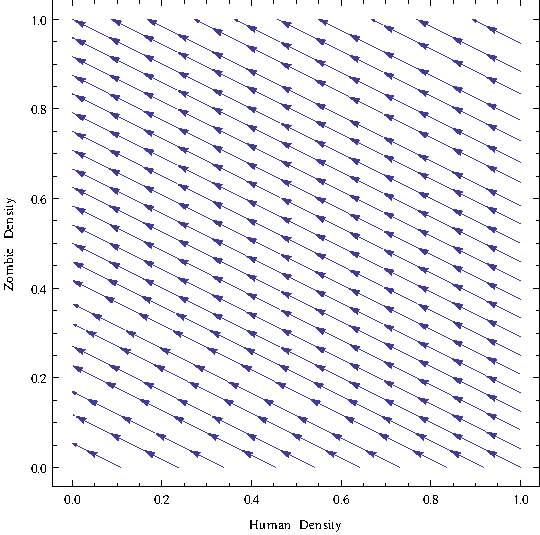
\includegraphics[width=0.4\linewidth]{images/phaseSpacePortraits/zombiesBeatHumans2to1} & 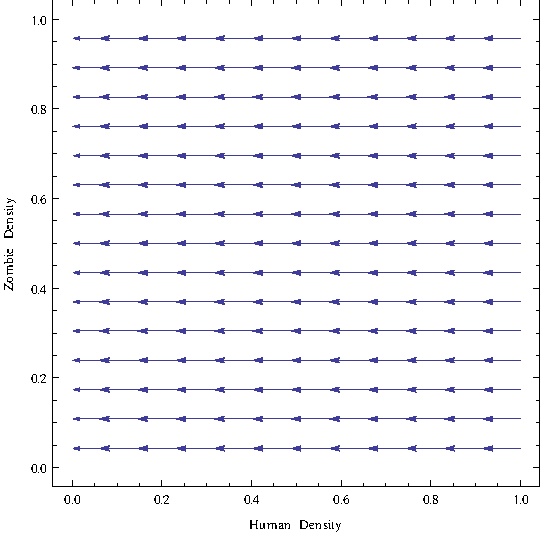
\includegraphics[width=0.4\linewidth]{images/phaseSpacePortraits/evenStevens} \\
    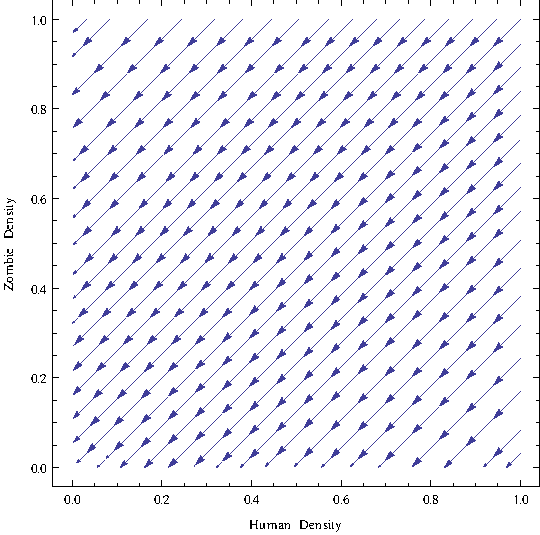
\includegraphics[width=0.4\linewidth]{images/phaseSpacePortraits/humansBeatZombies2to1} & 
\includegraphics[width=0.4\linewidth]{images/phaseSpacePortraits/cutLeonidas} \\
    $\alpha_H > \alpha_Z$ & Visualization of $\alpha_H > \alpha_Z$
    \end{tabular}
   }
   
   \headerbox{Simulation Results: The Plight of the The Three Towns}{name=results,column=2, row=0, span=2}{
%%%%%%%%%%%%%%%%%%%%%%%%%%%%%%%%%%%%%%%%%%%%%%%%%%%%%%%%%%%%%%%%%%%%%%%%%%%%%%
  In order to demonstrate that our model makes sense, we have simulated a specific case study using an explicit finite difference scheme.
  Here, the action is confined to a square,
  where reflecting boundary conditions have been used to ensure that zombies and humans do not leave the domain.
  Zombie combat efficacy $\alpha_Z$ is held at 1, whilst their rage $\sigma_Z$ is held at 2.5; both species' diffusion constants $\kappa$ are pinned
  at 1 for the duration, whilst human combat efficacy $\alpha_H$ and fear $\sigma_H$ vary with time $t$ as \\
  \begin{equation}
    \alpha_H = 2(1-e^{-\frac{t}{\tau_f}})
    \qquad
    \sigma_H = 7.5(1-e^{-\frac{t}{\tau_f}}) 
  \end{equation}
  where $\tau_f$ is the characteristic fightback time (=145 video frames; 400 in total) In the film clips below, 1 image is taken every 50 frames.
  The human density is shown first, with the zombie density below.
  \\
  \drawvideo{9}{100}{
   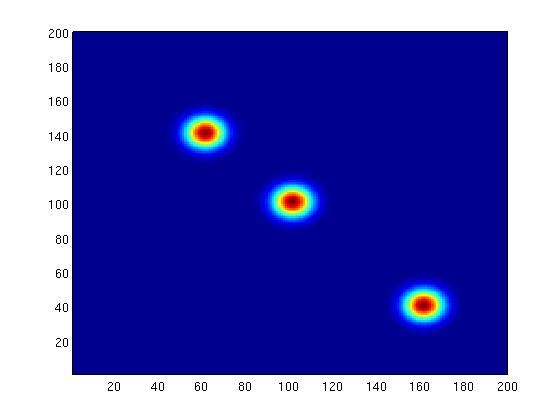
\includegraphics[width=0.103\linewidth]{images/someTowns/humanFrames/humans2}
   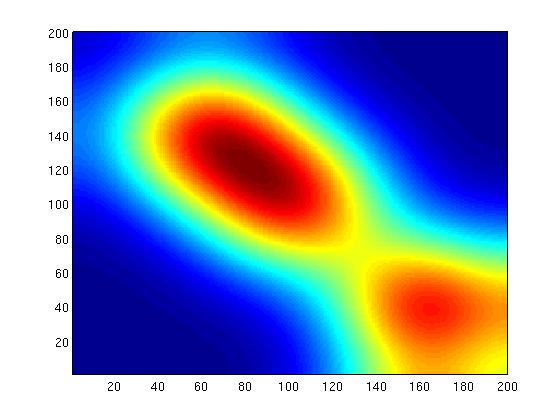
\includegraphics[width=0.103\linewidth]{images/someTowns/humanFrames/humans50}
   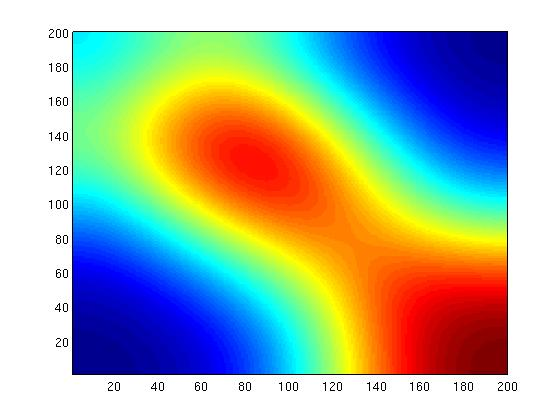
\includegraphics[width=0.103\linewidth]{images/someTowns/humanFrames/humans100}
   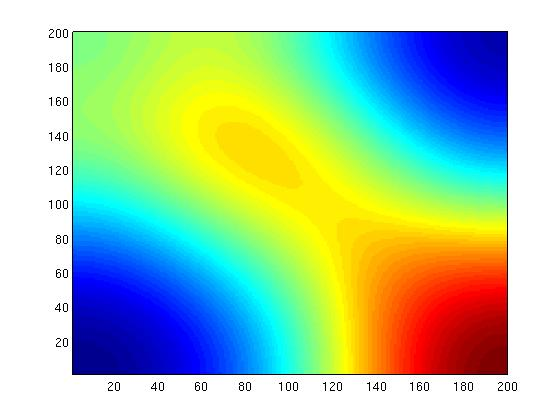
\includegraphics[width=0.103\linewidth]{images/someTowns/humanFrames/humans150}
   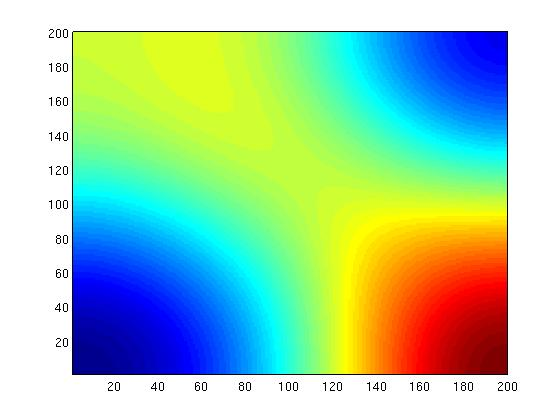
\includegraphics[width=0.103\linewidth]{images/someTowns/humanFrames/humans200}
   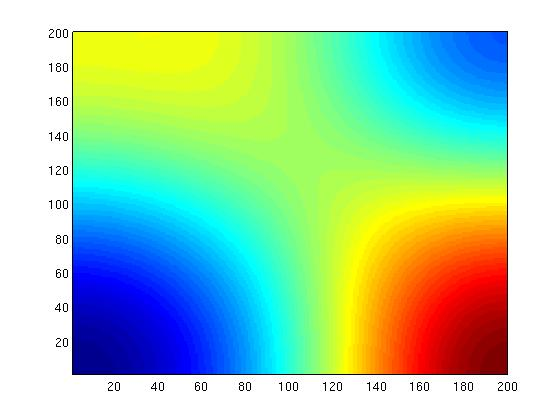
\includegraphics[width=0.103\linewidth]{images/someTowns/humanFrames/humans250}
   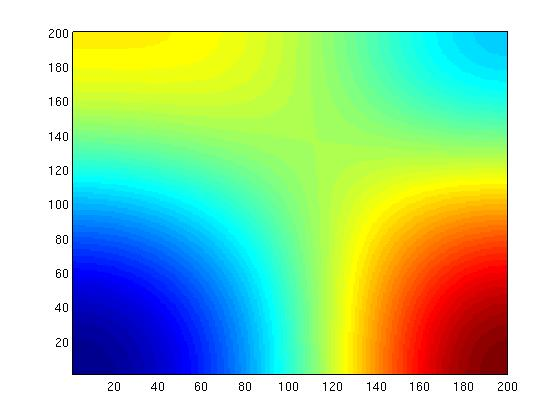
\includegraphics[width=0.103\linewidth]{images/someTowns/humanFrames/humans300}
   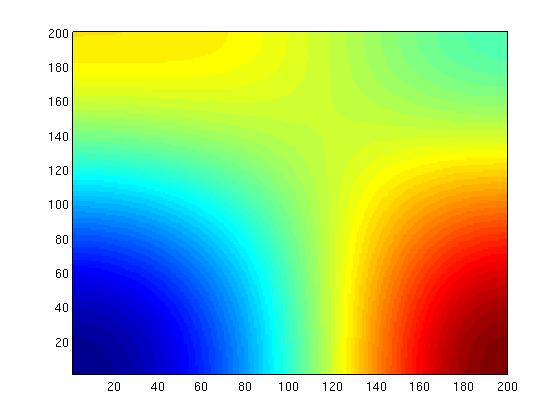
\includegraphics[width=0.103\linewidth]{images/someTowns/humanFrames/humans350}
   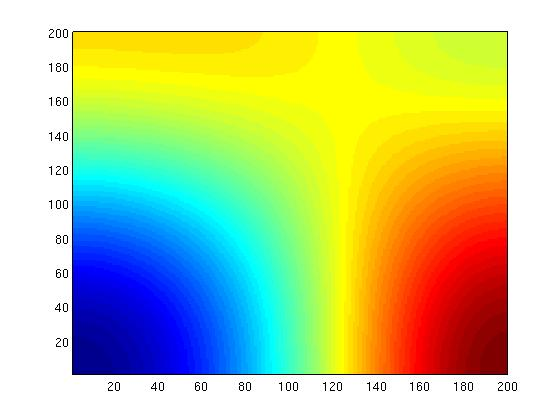
\includegraphics[width=0.103\linewidth]{images/someTowns/humanFrames/humans400}
  }
  \drawvideo{9}{100}{
   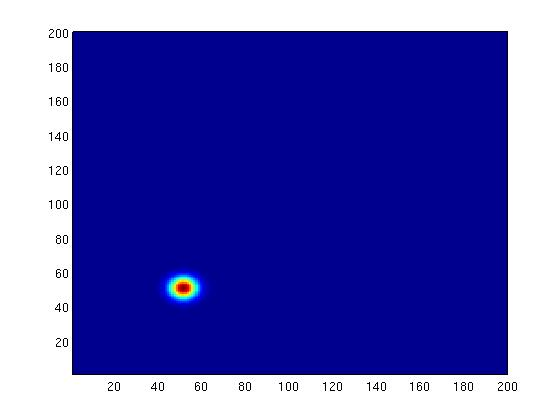
\includegraphics[width=0.103\linewidth]{images/someTowns/zombieFrames/zombies1}
   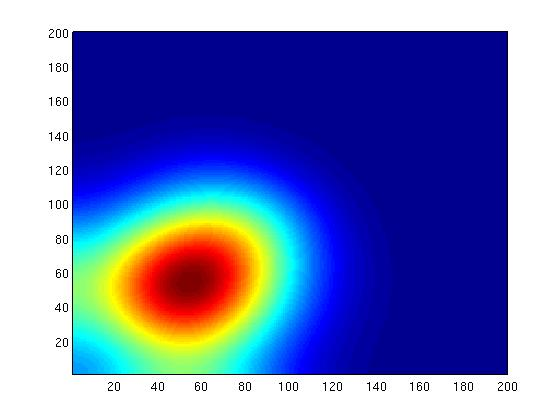
\includegraphics[width=0.103\linewidth]{images/someTowns/zombieFrames/zombies50}
   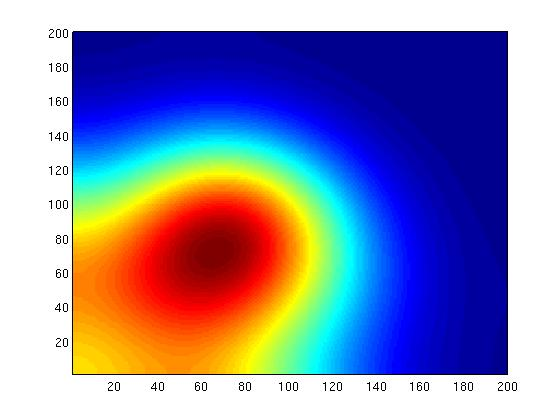
\includegraphics[width=0.103\linewidth]{images/someTowns/zombieFrames/zombies100}
   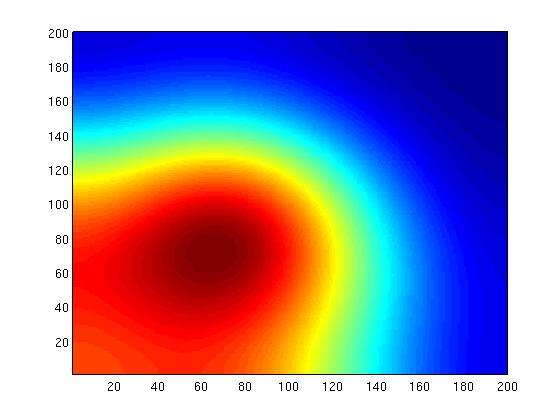
\includegraphics[width=0.103\linewidth]{images/someTowns/zombieFrames/zombies150}
   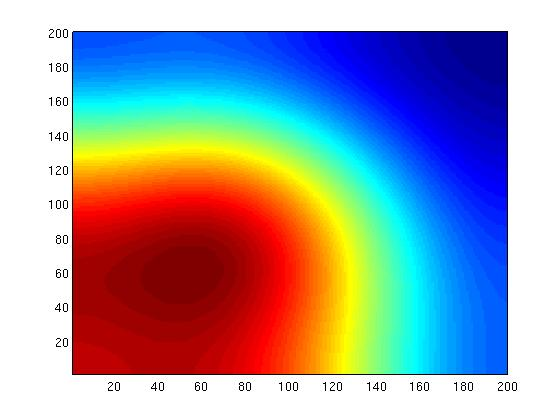
\includegraphics[width=0.103\linewidth]{images/someTowns/zombieFrames/zombies200}
   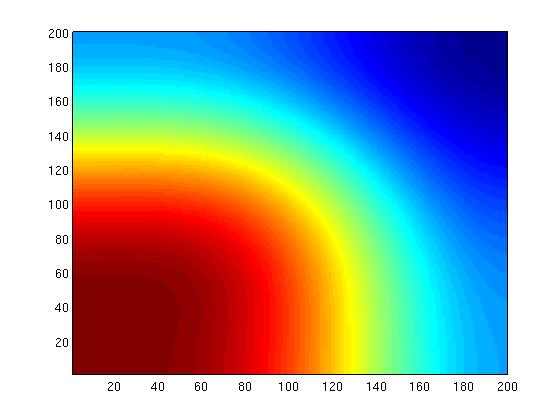
\includegraphics[width=0.103\linewidth]{images/someTowns/zombieFrames/zombies250}
   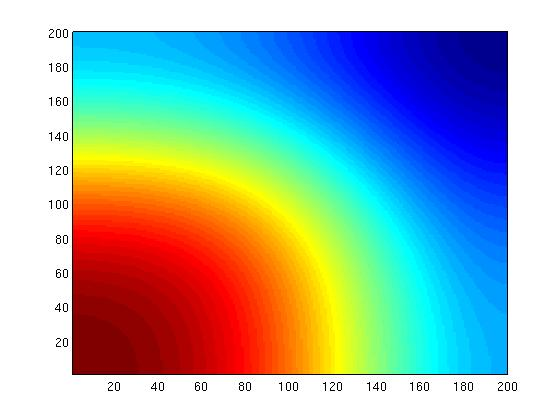
\includegraphics[width=0.103\linewidth]{images/someTowns/zombieFrames/zombies300}
   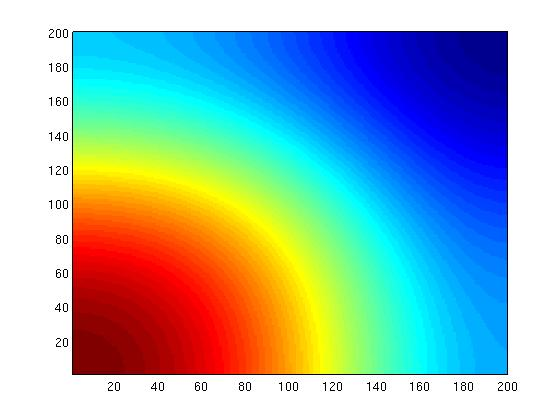
\includegraphics[width=0.103\linewidth]{images/someTowns/zombieFrames/zombies350}
   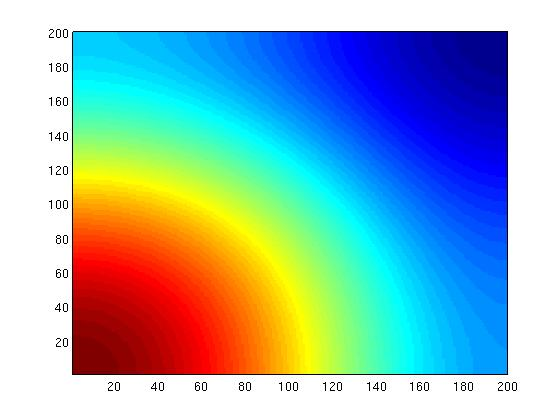
\includegraphics[width=0.103\linewidth]{images/someTowns/zombieFrames/zombies400}
  }
  \\
  \begin{minipage}[b]{0.33\linewidth}
   The left graph is the total human population over time; right is the total zombie population.
   Notice that the zombie population initially increases fairly rapidly, but then starts to
   decline as humans become more effective at killing zombies.
   \end{minipage}
   \begin{minipage}[t]{0.33\linewidth}
   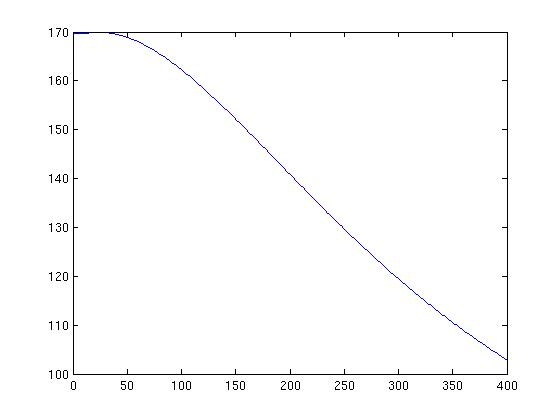
\includegraphics[width=\linewidth]{images/someTowns/humanPop}
   \end{minipage}
   \begin{minipage}[t]{0.33\linewidth}
   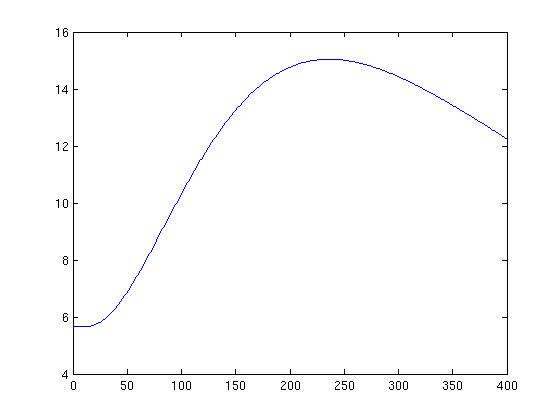
\includegraphics[width=\linewidth]{images/someTowns/zombiePop}
   \end{minipage}
  }
  \headerbox{Conclusions, Further Work and Acknowledgements}{name=conclusions,column=2, above=bottom, below=results, span=2}{
%%%%%%%%%%%%%%%%%%%%%%%%%%%%%%%%%%%%%%%%%%%%%%%%%%%%%%%%%%%%%%%%%%%%%%%%%%%%%%
  The zombie-human field theory developed here seems to capture some of the phenomena commonly observed in
  zombie films. However, there are some issues which would need to be addressed if we were to carry this research further:
  \begin{enumerate}
  \compresslist
   \item The finite-difference simulations do not appear to be stable unless sufficiently large diffusion parameters are used.
   Therefore we have not been able to explore the low-diffusion limit properly. This may be happening due to shock formation
   (which finite-difference would not be able to handle) or because the PDE system genuinely has inherent instability.
   \item The RHS of the equations seems to be unrealistic, as a group of humans fighting two batches of zombies sustains
   just as many losses as a group fighting both batches combined. Thus it may be prudent to consider some different models.
  \end{enumerate}
  I'd like to thank my group (Andrej Markovic, Peter Wu, Kaitai Dong and Faizan Fahmi) as well as everyone else on the Applied MSc course
  whose discourses have helped make this model. I would also like to thank all the PhD students who have contributed, as well as Brian
  Amberg whose poster template made this possible (and James Fielder for finding it, of course!).
  }
 
  
  \end{poster}
  
  \end{document}